%The \introduction command is provided as a convenience.
%if you want special chapter formatting, you'll probably want to avoid using it altogether
		
\chapter*{Introduction}
    \addcontentsline{toc}{chapter}{Introduction}
		\chaptermark{Introduction}
		\markboth{Introduction}{Introduction}
% The three lines above are to make sure that the headers are right, that the intro gets included in the table of contents, and that it doesn't get numbered 1 so that chapter one is 1.

	The study of pattern formation is incredibly diverse and certainly one of the most compelling aspects of nonlinear phenomenology. Scientists from many disciplines have analyzes patterns on the scale of the entire universe all the way down to the microscopic\footnote{See the introduction of Cross \& Greenside for an overview of the study of pattern formation.}. Just a cursory glance at the structure of a wind-swept sand dune, a snowflake, or even our own galaxy reveals something interesting. Observation of these patterns might lead a scientist to ask what causes the pattern and wonder why there are patterns at all. This question gets complicated quickly because whether it's God in the patterns or the result of a non-equilibrium universe, there is still the question of what it means to have ``structure'' or ``complexity'' or to be ``interesting''.
	
	Fortunately, the theoretical model of pattern formation discussed here allows me to sidestep all of these questions while focusing primarily on the method of analysis. There are many mathematical tools available to help interpret image data but as the complexity of our information (i.e.\ size of our data) increases, it becomes increasingly difficult to parse relevant information. Take for example the Fourier transform, a powerful method for image analysis. We would expect the Fourier transform to provide some insight into the spatial frequency of the image\footnote{In this case, the Fourier transform converts from the \textit{spatial domain}, the image we see, to the \textit{frequency domain}. The Fourier transform is often used to remove noise or apply filters to images. It has also been used for intricate pattern recognition, see\rf{hui_2014}.}. Examine the two distinct pattern types of the Gray-Scott system shown in \refFig{fig:fourierfail}. The two pattern types $\alpha$ and $\kappa$ (\reffigs{fig:alphagrey}{fig:kappagrey} respectively) are visually extremely distinct yet the Fourier transforms (\reffigs{fig:alphafft}{fig:kappafft}) are disappointingly similar. Although this method could certainly extract useful information, we would like some way to supplement our findings. The need for new methods arises and many times that means starting at the lowest level. The homology theory described later on considers the fundamental geometric structures of an image while providing insight into global properties.
	
\begin{figure}[h]
        \centering
        \begin{subfigure}[b]{0.3\textwidth}
                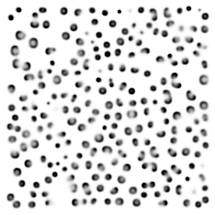
\includegraphics[width=\textwidth]{alpha_v_grey.png}
                \caption{Pattern type $\alpha$.}
                \label{fig:alphagrey}
        \end{subfigure} \quad
        \begin{subfigure}[b]{0.3\textwidth}
                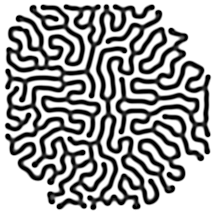
\includegraphics[width=\textwidth]{kappa_v_grey.png}
                \caption{Pattern type $\kappa$.}
                \label{fig:kappagrey}
        \end{subfigure} \\
        ~ %add desired spacing between images, e. g. ~, \quad, \qquad, \hfill etc.
          %(or a blank line to force the subfigure onto a new line)
          
        \begin{subfigure}[b]{0.3\textwidth}
                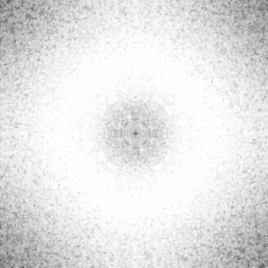
\includegraphics[width=\textwidth]{alpha_v_fft.png}
                \caption{Fourier-Transform of $\alpha$.}
                \label{fig:alphafft}
        \end{subfigure} \quad
        \begin{subfigure}[b]{0.3\textwidth}
                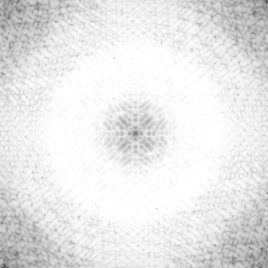
\includegraphics[width=\textwidth]{kappa_v_fft.png}
                \caption{Fourier-Transform of $\kappa$.}
                \label{fig:kappafft}
        \end{subfigure}
        \caption{For two very distinct pattern types $\alpha$ and $\kappa$, the Fourier-Transform is visually very similar and extracting meaningful information is difficult.}\label{fig:fourierfail}
\end{figure}